\section{Auswertung}
\label{sec:Auswertung}

\subsection{Wheatstonesche Brücke}
Mit der Wheatstoneschen Brücke (Abb: \ref{fig:wheatstonebrücke}) sollen zwei unbekannte Widerstände bestimmt werden.
Für den unbekannten Widerstand $R_x$ gilt nach Formel \eqref{eqn:widerstand}
\begin{equation}
	R_x = R_2 \frac{R_3}{R_4}
\end{equation}
Der erste bestimmte unbekannte Widerstand war der Widerstand 13.
	\begin{table}
		\centering
		\caption{Messdaten für Wert 13}
		\label{tab:wheat1}
	\begin{tabular}{cccc}
		\toprule
		$R_2$ / $\Omega$ & $R_3$ / $\Omega$ & $R_4$ / $\Omega$ & $R_x$ / $\Omega$ \\
		\midrule
		332 & 491,8 & 508,2 & 321,3 \pm 1,7 \\
		664 & 325,6 & 674,4 & 320,6 \pm 1,7 \\
		1000 & 242,9 & 757,1 & 320,8 \pm 1,7 \\
		\bottomrule
	\end{tabular}
	\end{table}

Die Messwerte mit dem berechneten Widerstand 13 sind in Tabelle \ref{tab:wheat1} dargestellt.
Für den Referenzwiderstand $R_2$ soll ein Fehler von $0,2\%$ und für das Verhältnis $\frac{R_3}{R_4}$ ein Fehler von $0,5\%$ angenommen werden (\cite{Anleitung}).
Daraus ergeben sich die Fehler für $R_x$ mit der Gaußschen Fehlerfortpfplanzung.

Damit ergibt sich für den zu bestimmenden Widerstand $R_{13} = (320,9 \pm 1,7??) \Omega$.
\newpage
Der zweite bestimmte Widerstand war der Widerstand 12.

	\begin{table}
		\centering
		\caption{Messdaten für Wert 12}
		\label{tab:wheat2}
	\begin{tabular}{cccc}
		\toprule
		$R_2$ / $\Omega$ & $R_3$ / $\Omega$ & $R_4$ / $\Omega$ & $R_x$ / $\Omega$ \\
		\midrule
		332 & 542,1 & 457,9 & 393,0 \pm 2,1 \\
		664 & 371,8 & 628,2 & 393,0 \pm 2,1 \\
		1000 & 282.0 & 718,0 & 392,8 \pm 2,1 \\
		\bottomrule
	\end{tabular}
	\end{table}
Die Messwerte und der ermittelte Widerstand $R_{12}$ sind in Tabelle \ref{tab:wheat2} dargestellt.

Für den zu bestimmenden Widerstand ergibt sich $R_{12} = (392,9 \pm 2,1??) \Omega$.

\subsection{Kapazitätsmessbrücke}
Der Aufbau einer Kapazitätsmessbrücke ist in Abbildung \ref{fig:kapazitätsmessbrücke} dargestellt.
Zunächst sollen die Widerstände einer RC-Kombination bestimmt werden.
Für den ohmschen Widerstand $R_x$ gilt nach Formel \eqref{eqn:kapwiderstand}$R_x = R_2 \frac{R_3}{R_4}$
Für den kapazitiven Widerstand $C_x$ gilt nach Formel \eqref{eqn:kapazitaet} $C_x = C_2 \frac{R_4}{R_3}$
	\begin{table}
		\centering
		\caption{Messdaten für das RC-Kombinations-Glied 8}
		\label{tab:kapakombi}
	\begin{tabular}{cccccc}
		\toprule
		$C_2$ / $nF$ & $R_2$ / $\Omega$ & $R_3$ / $\Omega$ & $R_4$ / $\Omega$ & $R_x$ / $\Omega$ & $C_x$ / $nF$ \\
		\midrule
		597 & 225,2 & 717,0 & 283,0 & 570,6 \pm 3,1 & 235,6 \pm 1,3 \\
		750 & 279,9 & 671,8 & 328,2 & 572,9 \pm 3,0 & 366,4 \pm 2,0 \\
		994 & 167,2 & 773,4 & 226,6 & 570,7 \pm 3,3 & 291,2 \pm 1,6 \\
		\bottomrule
	\end{tabular}
	\end{table}
Die Werte für das RC-Kombinations-Glied sind in Tabelle \ref{tab:kapakombi} dargestellt.
Der Fehler von $R_2$ wurde auf $\Delta R_2 = 0,5 \Omega$ festgelegt.

Damit erhält man für die zu bestimmenden Größen: $R_x = (571,4 \pm 3,1??) \Omega$ und $C_x = (297,7 \pm 1,6??) nF$.



Nun sollen die Kapazitäten zweier Kondensatoren bestimmt werden.
Hierfür wurden Die Kondensatoren 1 und 3 verwendet.
Es wurden jeweils der Kondensator $C_2$ variiert und der ohmsche Widerstand $R_2$ wurde auf Null gesetzt.

	\begin{table}
		\centering
		\caption{Messdaten für den Kondensator 1}
		\label{tab:kapa1}
	\begin{tabular}{ccccc}
		\toprule
		$C_2$ / $nF$ & $R_2$ / $\Omega$ & $R_3$ / $\Omega$ & $R_4$ / $\Omega$ & $C_x$ / $nF$ \\
		\midrule
		597 & 0 & 476,9 & 523,1 & 654,8 \pm 3,5 \\
		750 & 0 & 529,8 & 470,2 & 665,6 \pm 3,6 \\
		994 & 0 & 602,7 & 397,3 & 655,2 \pm 3,5 \\
		\bottomrule
	\end{tabular}
	\end{table}

Die Werte für den Kondensator 1 sind in Tabelle \ref{tab:kapa1} dargestellt.


	\begin{table}
		\centering
		\caption{Messdaten für den Kondensator 3}
		\label{tab:kapa3}
	\begin{tabular}{ccccc}
		\toprule
		$C_2$ / $nF$ & $R_2$ / $\Omega$ & $R_3$ / $\Omega$ & $R_4$ / $\Omega$ & $C_x$ / $nF$ \\
		\midrule
		597 & 0 & 589,1 & 410,9 & 416,4 \pm 2,2 \\
		750 & 0 & 639,5 & 360,5 & 422,8 \pm 2,3 \\
		994 & 0 & 704,9 & 295,1 & 416,1 \pm 2,2 \\
		\bottomrule
	\end{tabular}
	\end{table}
Die Werte für den Kondensator 3 sind in Tabelle \ref{tab:kapa3} dargestellt.


\subsection{Induktivitätsmessbrücke}


Die Induktivitätsmessbrücke ist in Abbildung \ref{fig:induktivitätsmessbrücke} dargestellt.
Die unbekannte Induktivität $L_x$ ($L_{17}$) wurde mittels Formel \eqref{eqn:induktivität} bestimmt, der
Verlustwiderstand $R_x$ ($R_{17}$) mit Formel \eqref{eqn:indukwiderstand}.

	\begin{table}
		\centering
		\caption{Messdaten für das L-R-Kombinationsglied 17}
		\label{tab:induk}
	\begin{tabular}{cccccc}
		\toprule
		$L_2$ / $mH$ & $R_2$ / $\Omega$ & $R_3$ / $\Omega$ & $R_4$ / $\Omega$ & $R_x$ / $\Omega$ & $L_x$ / $mH$ \\
		\midrule
		20,1 & 38,8 & 680,1 & 319,9 & 82,5 \pm 2,5 & 42,7 \pm 0,2 \\
		27,5 & 60,5 & 609,2 & 390,8 & 94,3 \pm 2,5 & 42,9 \pm 0,2 \\
		14,6 & 33,3 & 749,2 & 250,8 & 99,5 \pm 3,0 & 43,6 \pm 0,2 \\
		\bottomrule
	\end{tabular}
	\end{table}

Die Werte für das L-R-Kombinationsglied sind in Tabelle \ref{tab:induk} dargestellt.
Der Fehler von $R_x$ und $L_x$ durch die fehlerbehafteten Größen $L_2$ (0,2 \%), $R_2$ (3 \%) und $\frac{R_3}{R_4}$ (0,5 \%) wurden mittels Gaußscher Fehlerfortpfplanzung bestimmt.


\subsection{Maxwell-Brücke}

	\begin{table}
		\centering
		\caption{Messdaten für das L-R-Kombinationsglied 17}
		\label{tab:maxwk}
	\begin{tabular}{cccccc}
		\toprule
		$R_2$ / $\Omega$ & $C_4$ / $nF$ & $R_3$ / $\Omega$ & $R_4$ / $\Omega$ & $R_x$ / $\Omega$ & $L_x$ / $mH$ \\
		\midrule
		332 & 597 & 215,2 & 754,1 & 94,7 \pm 4,0 & 42,7 \pm 1,3 \\
		664 & 597 & 108,0 & 753,2 & 95,2 \pm 4,0 & 42,8 \pm 1,3 \\
		1000 & 597 & 72,0 & 753,2 & 95,6 \pm 4,1 & 43,0 \pm 1,3 \\
		\bottomrule
	\end{tabular}
	\end{table}


%Soll hier noch erklärung und verweis auf formeln hin?


\subsection{Wien-Robinson-Brücke}
In der letzten Messreihe soll die Frequenzabhängigkeit der Wien-Robinson-Brücke im Bereich $20Hz-30000Hz$ untersucht. Nach Abbildung \ref{fig:wheatstonebrücke} wurden Bauelemente mit den folgenden Kenndaten verwendet.

\begin{table}
\centering
\caption{Kenndaten der verwendeten Bauteile der Wien-Robinson-Brücke}
\begin{tabular}{cccc}
$R'$/$\Omega$& $2R'$/$\Omega$& $R$/$\Omega$ &$C_1$/$nF$\\
332&664&1000&	???

\end{tabular}
\end{table}
Die Kapazität des Kondensators $C_1$ wurde hierbei als Mittelwert der Berechnung in Tabelle \ref{tab:kapa1} angenommen.
In der nachfolgenden Tabelle sind die gemessenen Spannungen $U_s$, $U_Br, eff$ in Abhängigkeit zur Frequenz
$f$ sowie sowohl der gemessene Quotient der Spannungen als auch der nach
Formel \eqref{eqn:wienquotient} berechnete Quotient eingetragen. Zudem wird $\Omega =\frac{f}{f_0}$ aufgeführt.
Da es sich um eine Wechselspannung handelt, berechnet sich $U_Br, eff$ nach
\begin{equation}
	U_Br, eff=\frac{U_Br}{2 \sqrt{2}}
\end{equation}
und $\omega_0$ ist die Frequenz, bei der die Brückenspannung verschwindet.
Da
\begin{equation}
	v_0=\frac{\omega_0}{2 \pi}; mit \omega_o=\frac{1}{RC}
\end{equation}
Bei unserem Aufbau ergab sich $\omega_0$ etwa zu $240Hz$. Nach der Formel würde sich etwa $\omega_0=241.6Hz$ ergeben.
\begin{table}
  \label{tab:wien}
  \centering
  \caption{Messdaten}
\begin{tabular}{cccccc}
  \toprule
$\omega \si{\Hz}$ & $U_\text{S}$ / $\Omega$ & $U_{\text{Br, eff}}$/$\si{\milli\ohm}$ & $\frac{U_{\text{Br}}}{U_S}$ nach \eqref{eqn:wienquotienteinfach} & $\frac{U_{\text{Br}}}{U_\text{S}}$ & $\frac{\omega}{\omega_0}$ \\
\midrule
20.0 & 2.82 & 1979.90 & 0.3510 & 0.3234 & 0.08 \\
70.0 & 2.85 & 1414.21 & 0.2481 & 0.3174 & 0.29 \\
110.0 & 3.00 & 1018.23 & 0.1697 & 0.3082 & 0.46 \\
140.0 & 3.00 & 714.18 & 0.1190 & 0.2943 & 0.58 \\
170.0 & 2.99 & 438.41 & 0.0733 & 0.2741 & 0.70 \\
190.0 & 2.97 & 292.74 & 0.0493 & 0.2463 & 0.79 \\
200.0 & 2.98 & 234.76 & 0.0394 & 0.2104 & 0.83 \\
210.0 & 2.99 & 173.95 & 0.0291 & 0.1670 & 0.87 \\
220.0 & 2.95 & 106.07 & 0.0180 & 0.1181 & 0.91 \\
225.0 & 2.95 & 74.95 & 0.0127 & 0.0658 & 0.93 \\
230.0 & 2.93 & 42.43 & 0.0072 & 0.0120 & 0.95 \\
235.0 & 2.92 & 22.06 & 0.0038 & 0.0421 & 0.97 \\
240.0 & 2.93 & 11.88 & 0.0020 & 0.0953 & 0.99 \\
245.0 & 2.95 & 27.15 & 0.0046 & 0.1460 & 1.01 \\
250.0 & 2.95 & 62.23 & 0.0105 & 0.1920 & 1.03 \\
255.0 & 2.96 & 86.97 & 0.0147 & 0.2314 & 1.06 \\
260.0 & 2.95 & 109.60 & 0.0186 & 0.2628 & 1.08 \\
270.0 & 2.96 & 157.68 & 0.0266 & 0.2863 & 1.12 \\
280.0 & 2.92 & 210.72 & 0.0361 & 0.3027 & 1.16 \\
290.0 & 2.91 & 258.80 & 0.0445 & 0.3138 & 1.20 \\
310.0 & 2.85 & 323.85 & 0.0568 & 0.3211 & 1.28 \\
340.0 & 2.84 & 434.16 & 0.0764 & 0.3257 & 1.41 \\
370.0 & 2.72 & 534.57 & 0.0983 & 0.3286 & 1.53 \\
500.0 & 2.69 & 869.74 & 0.1617 & 0.3304 & 2.07 \\
750.0 & 2.64 & 1223.29 & 0.2317 & 0.3315 & 3.10 \\
1000.0 & 2.62 & 1400.07 & 0.2672 & 0.3322 & 4.14 \\
3000.0 & 2.60 & 1697.06 & 0.3264 & 0.3327 & 12.42 \\
7000.0 & 2.62 & 1739.48 & 0.3320 & 0.3329 & 28.97 \\
12000.0 & 2.63 & 1704.13 & 0.3240 & 0.3331 & 49.67 \\
20000.0 & 2.67 & 1668.77 & 0.3125 & 0.3332 & 82.78 \\
30000.0 & 2.69 & 1598.06 & 0.2970 & 0.3332 & 124.17 \\
\end{tabular}
\end{table}

\begin{figure}
	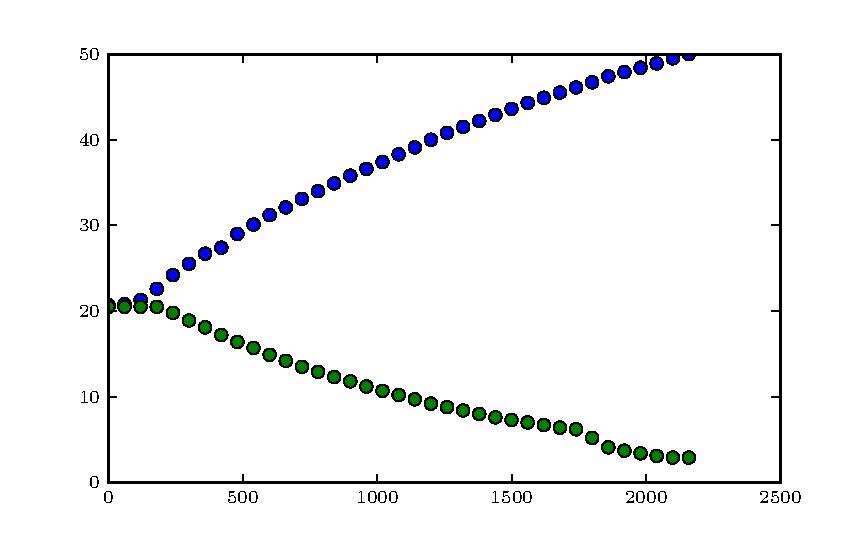
\includegraphics{build/plot.pdf}
	\caption{Vergleich der Messdaten mit der Theoriekurve}
	\label{fig:plot1}
\end{figure}
\subsubsection{Klirrfaktor-Messung}
Wie bereits in der Theorie beschrieben, wird im vorliegenden Experiment die Näherung
verwendet, dass lediglich die zweite Oberwelle betrachtet wird.
Zur Berechnung von $k$ nach Formel \eqref{eqn:klirrfaktor} werden also $U_1$ und $U_2$ benötigt. $U_1$ ist $U_S=2.93 \Omega$ bei $\omega_0$. Mit \eqref{eqn:wienquotienteinfach} und $\Omega=2$ sowie
\begin{equation}
	\label{eqn:klirrfkt}
U_2=\frac{U_{Br}}{f(2)}
\end{equation}
f(2) ist, mit \Omega=2, hierbei:
\begin{equation}
f(2)^2=\left|\frac{U_Br}{U_s}\right|^2(\Omega)=\frac{1}{45}
\end{equation}
Damit ergibt sich $U_2=0.079 \Omega$ und schließlich
\begin{equation}
k=\frac{U_2}{U_1}=0.027
\end{equation}
Formel \eqref{eqn:klirrfkt} wurde nach \cite{Anleitung} verwendet.
